\chapter{Lexical Cohesion Graph}
\label{chapt:lexical_coherence_graph}


\section{Introduction}
\label{sec:introduction}
The concept of coherence is based on cohesive semantic relations
connecting elements of a text. 
Cohesive relations are expressed through grammar and the vocabulary of a language. 
The former is referred to as \emph{grammatical coherence}, the latter as \emph{lexical coherence}\ \cite{halliday76}. 
Grammatical coherence encompasses coreference, substitution, ellipsis, etc. 
For instance, the entity graph model is mainly based on entities that are defined as coreferent mentions in a document.  
Lexical coherence comprises semantic connections among words of a text.
In this chapter, we measure text coherence by modeling \emph{lexical coherence} that is 
built on semantic relations between words of sentences of a text. 
Lexical relations can be any kinds of semantic relation: 

\begin{itemize}
\item repetition that happens when a word of a sentence is repeated in another sentence;

\item synonymy that happens when a word of a sentence means exactly or nearly the same as a word in another sentence. 
For example, verbs ``buy'' and ``purchase'' have synonymy relation;  

\item hyperonymy that shows the relationship between a generic word (hypernym) in a sentence and a specific instance of it (hyponym) in another sentence. 
For example, words ``red'', ``blue'' and ``color'' are semantically related because they have hyperonymy relation;

\item meronymy that happens when a word of a sentence is a constituent part of, or a member of a concept that is mentioned by a word in another sentence. 
For example, finger and hand have the meronymy relations because a finger is part of a hand;

\item ...
\end{itemize}

\cite{halliday76} explain that there is coherence between any pair of lexical items that stand to each other in some lexico-semantic relation, regardless of the relation type. 
Based on \cite{halliday76}, for the texture purposes it is only necessary to recognize semantically related lexical items. 
The other important point is that lexical items should not necessarily have the same reference \cite{halliday76}. 
Consider the following example: 

\begin{quote}
\emph{Why does the little boy wriggle all the time? Girls don't.}
\end{quote}

In this example the lexical items \emph{boy}\ and \emph{girls}\ are semantically related and make these two sentences related.  
They do not refer to the same entity, though. 

In order to recognize lexical semantic relations between words, we need to employ some world knowledge. 
One way to do this, is using a resources such as WordNet \cite{fellbaum98} or Freebase \cite{bollacker08}.  
This way is expensive in terms of determining the best resource.  
WordNet lacks broad coverage in particular with proper names, Freebase is restricted to nominal concepts and entities. 
In addition, they are rarely available for other languages than English.
If they are available, almost none of them come close to WordNet's size and coverage on English. 

The other way is to use word embeddings that are train a large corpora. 
Embedding representations of words let us efficiently compute semantic relations among lexical items in the vector space. 
Words that are semantically related in the text space, their embeddings are similar to each other in the vector space. 
These vectors can be easily trained for any language if a large corpus of documents on the language is available. 
The main advantage of word embeddings is that semantic relations between words can simply be computed by the cosine function and the semantic relations between words is relative.  
So we use word embeddings to check the existence of a semantic relations between two words. 

In the following example the sentences are connected because of the semantic relation between \emph{king}\ and \emph{queen}\ which can be induced by word embedding models \cite{mikolov13c,pennington14}.

\begin{quote}
  \emph{\ldots The king was in his counting-house, counting out his money,\\ 
    The queen was in the parlour, eating bread and honey.} 
\end{quote}


Since graph representations of entity-based relations across sentences in a document have been shown useful for modeling coherence, we propose to encode lexical relations among sentences in a document by a graph as well. 
We name our mode lexical coherence graph (LCG) that encodes if semantic relations between words of sentences.  
Therefore, the main contribution of this chapter is that we extends semantic relations between sentences from entity-based relations to lexical-based relations using word embeddings and propose a new approach for encoding these relations via graphs. 

Given lexical coherence graphs of documents in a dataset, similar to the previous chapter, we apply a subgraph mining algorithm to mine all patterns occurring in these graphs. 
We take subgraphs as coherence patterns and use their frequency as features representing the connectivity of the graph and, hence, the coherence of a document. 
Although using the frequency of subgraphs of the lexical coherence graph encodes coherence features well, the subgraph frequency method, in general, is suffering from a sparsity problem when the size of subgraphs increases. 
Large subgraphs capture more structural information, but they occur rarely in graph representations of documents.  
We resolve this sparsity issue by adapting \mbox{Kneser-Ney} smoothing \cite{heafield13} to smooth subgraph frequencies. 
We estimate the probability of unseen subgraphs with respect to similar subgraphs (in terms of connectivity style) that are seen before.  
This estimation enables our model to measure the coherence of a document even when its corresponding graph representation does not contain large subgraphs. 
If the unseen coherence pattern is similar to seen ones, smoothing gives it closer
probability to seen coherence patterns in comparison to dissimilar
unseen ones. 


In order to evaluate our model, we apply our coherence model to readability assessment task as an important task for coherence evaluation. 
The goal of this task is to rank documents with respects to their readability. 
The more coherent a text, the faster to read and easier to understand it is. 
We evaluate our LCG model on the two readability datasets provided by \newcite{pitler08} and \newcite{declercq14}. 
The results indicate that the LCG model outperforms \mbox{state-of-the-art} systems. 
By applying \mbox{Kneser-Ney} smoothing we solve the sparsity problem. 
Smoothing allows us to exploit the high informativity of large subgraphs which leads to new \mbox{state-of-the-art} results in readability assessment.
% Other coherence models \cite{barzilay08,guinaudeau13,mesgar14} are also evaluated on this
% task.
% \newcite{pitler08} use the entity grid \cite{barzilay08} to capture the coherence of a text for readability assessment. 
% \newcite{mesgar15} extend the entity graph \cite{guinaudeau13} as coherence model to measure the readability of texts. They encode coherence as a vector of
% frequencies of subgraphs of the graph representation of a text. 
% We build upon their method and represent the connectivity of sentences in our LCG model by a vector of frequencies of subgraphs.

We summarize the contributions of this chapter as follows:

\begin{itemize}

  \item Proposing a new \mbox{graph-based} representation of lexical semantic relations across sentences,

  \item Adapting \mbox{Kneser-Ney} smoothing approach in order to solve the sparsity problem in frequency of large coherence patterns,  

  \item Evaluating the model on two readability datasets \newcite{pitler08} and \newcite{declercq14}

\end{itemize}


\section{Lexical Cohesion Graph (LCG)}
\label{sec:lexical_coherence_graph}
In this section, we introduce a new graph representation of lexical semantic relations  across sentences in a document. 
We extract all occurring subgraphs in lexical graphs of documents in a dataset to obtain coherence patterns.  
Then we compute frequencies of coherence patterns in a lexical graph of a document to capture the connectivity style of the graph and therefore the perceived coherence of the document. 

\subsection{Graph Model} 
We model semantic relations between sentences by a graph
$G = < V, E > $ where $V$ is a set of nodes representing sentences in a document, and
$E$ is a set of directed edges. 
An edge between two nodes represents existence of a lexical semantic relation between the sentences and the direction of the edge indicates the sentence order in the document.   
Two sentences are semantically connected if there is at least one strong semantic relation between words of the sentences. 
Semantic relations between words are modeled by their corresponding pre-trained word embeddings \cite{pennington14}. 
Given word vectors $v_a$ for word $a$ of sentence $A$ and $v_b$ for word $b$ of sentence $B$, the cosine similarity value, $cos(v_a,v_b)$, between these two word vectors is a measure of semantic connectivity of words $a$ and $b$. 
The range of $cos(v_a,v_b)$ is between $\lbrace -1, +1 \rbrace$. 
One interpretation of cosine is the normalized correlation coefficient, which states how well its two input words are semantically correlated \cite{manning99}. 
The absolute value of cosine, $|cos(v_a,v_b)|$, encodes how strongly two words are
connected.

The connection between sentences is obtained from connections between their words (Figure \ref{f:wrd_rel}). 
Assume sentence $A$ precedes sentence $B$, each word $b$ of sentence $B$ is connected with word $a^\ast$ of $A$, where

\begin{equation*}
a^\ast= \argmax_{a\in A}cos(b,a)
\end{equation*}

\begin{figure}[!ht]
\centering
\small

\begin{tabular}{c}
\begin{tikzpicture}[shorten >=1pt,->,scale=0.62]

     \tikzstyle{word}=[circle,thick,draw=black!75,fill=black!10,minimum size=2mm]
     \tikzstyle{sent}=[ellipse, draw, minimum height=1.5cm]
        \tikzstyle{edge}=[draw, dashed,-]
       \begin{scope}  
         \node [word] (w1) at (0,0) {\tiny{$v_1$}};
         \node [word] (w2) at (2,0) {\tiny{$v_2$}};
         \node [word] (w3) at (4,0) {\tiny{$v_3$}}; 
          \node[sent, minimum width=4cm]  (A) at (2,0) {};         
    
    
         \node [word] (w4) at (8,0) {\tiny{$v_4$}}; 
         \node [word] (w5) at (10,0) {\tiny{$v_5$}}; 
         \node[sent, minimum width=3cm ] (B) at (9,0) {};         

         
         
         \path[edge , bend right=60] (w4) edge [above] node[font=\tiny] {} (w1);
         \path[edge, bend right=60, solid] (w4) edge [above] node[font=\tiny] {} (w2);
         \path[edge, bend right=60] (w4) edge [above] node[font=\tiny] {} (w3);
          
        
         \path[edge ,bend left=60] (w5) edge [above] node[font=\tiny] {} (w1);
         \path[edge,bend left=60] (w5) edge [above] node[font=\tiny] {} (w2);
         \path[edge,bend left=60, solid] (w5) edge [above] node[font=\tiny] {} (w3);
        \end{scope}        
      \end{tikzpicture}
\end{tabular}
\caption{Sentence A with three word vectors $\lbrace v_1,v_2,v_3 \rbrace$ and
  sentence B with two word vectors $\lbrace v_4, v_5 \rbrace$. 
  $v_4$ has the maximum similarity with $v_2$ and $v_5$ with $v_3$.} 
\label{f:wrd_rel}
\end{figure}

We consider $|cos(b,a^\ast)|$ as the weight of the edge that connects word $b$ of sentence $B$ to word $a^\ast$ of sentence $A$. 
We connect each word of $B$ with the most semantically related word of $A$. 
Then from all connections between the words of sentences $A$ and $B$, the connection with the maximum weight among the words of $B$ is selected to connect these two sentences (Figure \ref{f:sent_rel}) in lexical graph. 
We prune all edges whose weights are less than a threshold.  
We use threshold because the resulting graph is complete, we filter
out edges whose weights are below a threshold\footnote{We set this threshold to $0.9$ to connect only sentences with high confidence.}.


\begin{figure}[!ht]
\centering
\small

\begin{tabular}{c}
\begin{tikzpicture}[shorten >=1pt,->,scale=0.62]

     \tikzstyle{word}=[circle,thick,draw=black!75,fill=black!10,minimum size=2mm]
      \tikzstyle{sent}=[ellipse, draw, minimum height=1.5cm]
        \tikzstyle{edge}=[draw, dashed,-]
       \begin{scope}  
         \node [word] (w1) at (0,0) {\tiny{$v_1$}};
         \node [word] (w2) at (2,0) {\tiny{$v_2$}};
         \node [word] (w3) at (4,0) {\tiny{$v_3$}}; 
          \node[sent, minimum width=4cm]  (A) at (2,0) {};         
    
    
         \node [word] (w4) at (8,0) {\tiny{$v_4$}}; 
         \node [word] (w5) at (10,0) {\tiny{$v_5$}}; 
         \node[sent, minimum width=3cm ] (B) at (9,0) {};         

          
          \path[edge, bend right=60] (w4) edge  (w2);
          
          \path[edge, bend left=60, thick] (w5) edge (w3);
      \end{scope}        
  \end{tikzpicture}

\\
(a)

\\
      
  \begin{tikzpicture}[shorten >=1pt,->,scale=0.62]

     \tikzstyle{word}=[circle,thick,draw=black!75,fill=black!10,minimum size=2mm]
      \tikzstyle{sent}=[ellipse, draw, minimum height=1.5cm]
      \tikzstyle{edge}=[draw]
       \begin{scope}  
         \node [word] (w1) at (0,0) {\tiny{$v_1$}};
         \node [word] (w2) at (2,0) {\tiny{$v_2$}};
         \node [word] (w3) at (4,0) {\tiny{$v_3$}}; 
          \node[sent, minimum width=4cm]  (A) at (2,0) {};         
    
         \node [word] (w4) at (8,0) {\tiny{$v_4$}}; 
         \node [word] (w5) at (10,0) {\tiny{$v_5$}}; 
         \node[sent, minimum width=3cm ] (B) at (9,0) {};       
          
        \path[->, edge,bend right=60, thick] (A) edge  (B);
        \end{scope}        
  \end{tikzpicture}
    \\
    (b)
    \\
\end{tabular}


\caption{The word relation with the maximum weight (a) represents the connections between sentences (b).}
\label{f:sent_rel}
\end{figure}

\subsection{Coherence Features} 
\newcite{mesgar15} propose that the connection style of an entity
graph can be captured by the frequency of all \knode\ subgraphs in
this graph. Larger\footnote{The size of a subgraph is the number of
  its nodes.} subgraphs\footnote{We compute \emph{induced
    subgraphs} \cite{mesgar15}. However, we use the term
  \emph{subgraph} for brevity.} can capture more information about the
structure of graphs and are more informative coherence patterns than
smaller ones. We experiment with $k \in \{3,4,5,6\}$. Text coherence is
represented by a vector whose elements are the frequency of subgraphs
(coherence patterns) with \knode.

\subsection{Smoothing} 
% 
Although increasing the size $k$ of subgraphs captures more
structural information about the connections of sentence nodes, a
main risk with large subgraphs is sparsity. Given a sentence graph,
many large subgraph types do not occur in this graph.  Small subgraph
types occur frequently in most sentence graphs in the dataset, but
these subgraphs do not capture enough information about the
connectivity style of the graphs.

Inspired by Kneser-Ney smoothing in language models \cite{heafield13},
each feature vector of a sentence graph can be smoothed. Smoothing
deals with the problem of zero counts in the feature vector.  It also
lets the model having feature values for unseen subgraphs (like OOV in
language modeling) which may be seen in the testing phase.

\begin{figure*}[!t]
\centering
\small
%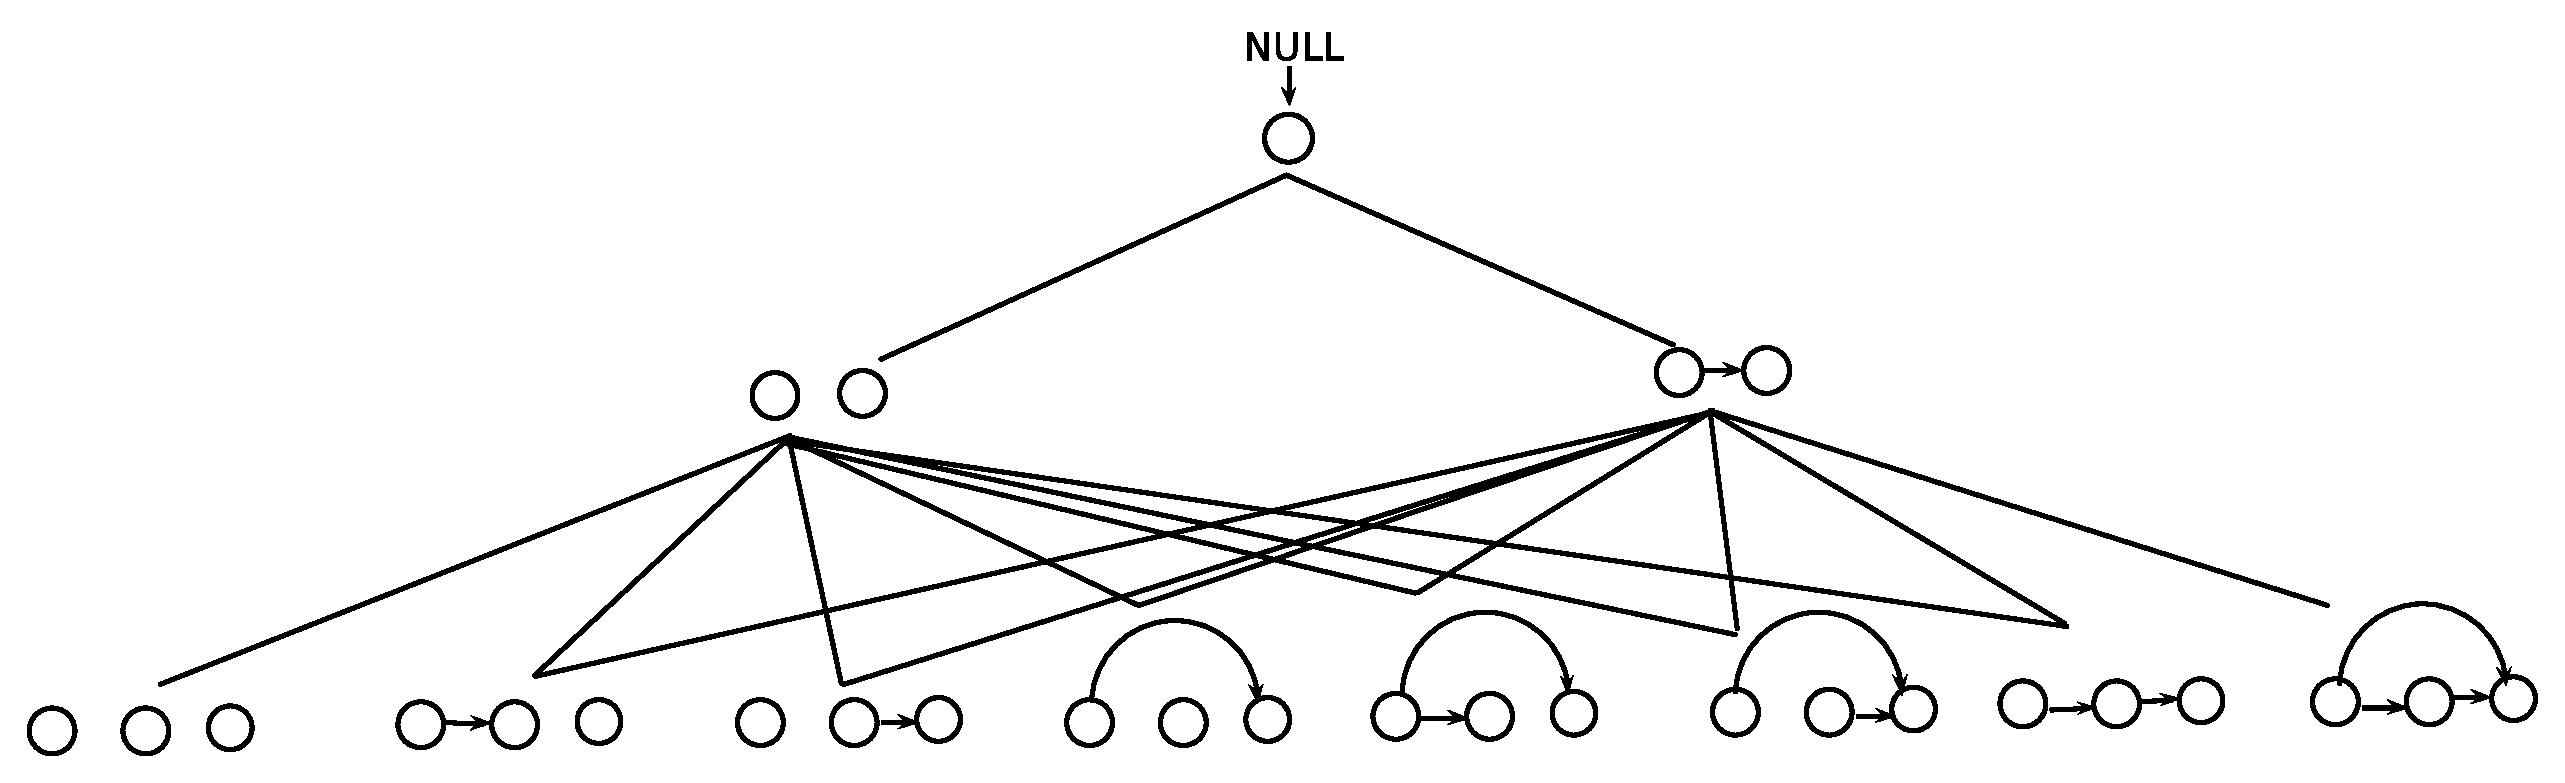
\includegraphics[scale=.38]{./figures/parent_child_relation.eps}
\caption{parent child relation.} 
\label{f:parent_child_rel}
\end{figure*}

Kneser-Ney smoothing uses a discount factor to discount the raw count
of each event (subgraph) and distributes the total discount to all
event (subgraph) probabilities by means of a base probability.

The estimated frequency of subgraph $sg$ in a given sentence graph
is computed as follows:

\begin{equation*}
KN(sg) = \frac{\max \lbrace	 count(sg)-\alpha, 0 \rbrace }{Z} + \frac{M \cdot \alpha}{Z}P_b(sg),
\end{equation*}
%
where $\alpha$ is the discount factor and $M$ is the number of times
that discount factor is applied. $Z$ is a normalization factor
to ensure that the distribution sums to one and is obtained as follows:

\begin{equation*}
Z = \sum_{sg \in A} count(sg),
\end{equation*}
%
where $A$ is the set of all subgraphs with \knodes\ and function
$count(\cdot)$ computes the number of instances of subgraph $sg$ in
the given sentence graph.

$P_b(sg)$ in Kneser-Ney smoothing is the base probability of
subgraph $sg$ among all \knode\ subgraphs ($A$). The base
probability can be computed based on hierarchical (parent-child)
relations in subgraphs. \knode\ subgraph $sg_i$ is a parent
of \kplusnode\ subgraph $sg_j$, if $sg_i$ is a subgraph of
$sg_j$. Figure \ref{f:parent_child_rel} shows the parent-child
relation between subgraphs via a weighted tree. The root of this tree
is a null graph
\footnote{A null graph is a graph with no nodes.}. 
The weight of a parent-child relation connecting the parent
subgraph $sg_i$ and child subgraph $sg_j$ is shown by $w_{ij}$ and
computed as follows:

\begin{equation*}
w_{ij} = \frac{count(sg_i, sg_j)}{\sum_{sg_l \in A}count(sg_i,sg_l)},
\end{equation*}
%
where $A$ is all subgraphs with \knode\ and $k$ equals the number of
nodes of $sg_j$. Interpretation of weight $w_{ij}$ is the normalized count of $sg_i$ in $sg_j$ with respect to all outgoing edges from $sg_i$.

The base probability of each subgraph $sg_j$ is the inner product
of the Kneser-Ney probabilities of $sg_j$'s parents by the weights of
the corresponding relations:

\begin{equation}
P_b(sg_j)  = P \cdot W,
\end{equation}
%
where $P$ is the vector of probabilities of all parents of 
$sg_j$ and $W$ is the vector of all corresponding edge weights
connecting the parents of $sg_j$ to $sg_j$.

Since the root node of this tree is the null subgraph, and it is a
subgraph of all possible sentence graphs, its base probability is
one. Because the edge weights are in the range $\left[0,1\right]$ the
sum of the probabilities of all subgraphs with \knode\ is always
equal to one.

\paragraph{Proof.} 
Assume $I$ and $J$ are the set of all \knode\ and \kplusnode\
subgraphs. We also assume that $I$ has $n$ subgraphs and $\sum_{i=1}^n
p(sg_i)=1$. Considering these assumptions we prove that

\begin{equation*}
\sum_{j=1}^m p(sg_j)=1,
\end{equation*}

\noindent
where $m$ is the number of subgraphs in $J$.

We start from the left and compute the value of 

\begin{equation*}
\sum_{j=1}^m p(sg_j).
\end{equation*}

\noindent
Based on the definition of base probability, the value of
$p(sg_j)$ is computed based on its parents in $I$,

\begin{equation*}
p(sg_j)=\sum_{i=1}^n w_{ij}p(sg_i),
\end{equation*}

\noindent
where $w_{ij}$ is the weight of the parent-child relation between
$sg_i$ and $sg_j$.  Now we have:

\begin{equation*}\sum_{j=1}^m p(sg_j) = \sum_{j=1}^m\sum_{i=1}^n w_{ij}p(sg_i).
\end{equation*}

\noindent
If we exchange the place of the sums and re-write the equation, we
have: 

\begin{equation*}
\sum_{j=1}^m p(sg_j) = \sum_{i=1}^n \sum_{j=1}^m w_{ij}p(sg_i).
\end{equation*}

\noindent
In this equation $p(sg_i)$ is independent of $j$ (index of the inner
sum), so it can be moved out of the inner sum:

\begin{equation*}
\sum_{j=1}^m p(sg_j) = \sum_{i=1}^n p(sg_i) \sum_{j=1}^m w_{ij}
\end{equation*}

\noindent
The inner sum equals $1$.

\begin{equation*}
\sum_{j=1}^m p(sg_j) = \sum_{i=1}^n p(sg_i).
\end{equation*}

\noindent
Based on our assumption the right side of the equation is $1$ and 

\begin{equation*}
\sum_{j=1}^m p(sg_j) = 1.
\end{equation*}

\noindent
So we proved that the sum of the base probability of all \knode\
subgraphs is $1$.\QEDB


This way, Kneser-Ney smoothing distributes the total discount value by
considering the weights of parent-child relations among the
subgraphs. The result of applying smoothing is an estimation of the
frequency of each subgraph in the sentence graph.



\section{Experiments}
\label{sec:experiments}

\footnote{We use threshold $0.9$. It means we capture the semantic connection confidentially}


\subsection{Readability Assessment}
\label{subsec:readability_assessment}
We evaluate our coherence model on the task of ranking texts by their
readability. The intuition is that more coherent texts are easier to
read. 


\subsubsection{Data}
\paragraph{Datasets.} We run our experiments on two datasets annotated
with readability information provided by human annotators: \emph{P\&N}\
\cite{pitler08} and \emph{De Clercq}\ \cite{declercq14}.

The dataset \emph{P\&N}\ contains 27 articles randomly selected from
the Wall Street Journal corpus%
%
\footnote{\newcite{pitler08}'s dataset contains 30 articles. They
  remove one. We assume this is \texttt{wsj\--0382} which
does not exist in the Penn Treebank. We furthermore remove
\texttt{wsj\--2090} which does not exist in the final release of the
Penn Discourse Treebank. We also remove \texttt{wsj\--1398} which is a
poem and, hence, not very informative for readability assessment.}%
%
. The average number of sentences is about $10$ words. Every article is
associated with a human score between $[0.0,5.0]$ indicating the
readability score of that article. We create pairs of documents, if
the difference between their readability scores is greater than
$0.5$. If the first document in a pair has the higher score, we label
this pair with $+1$, otherwise with $-1$. The resulting number of text pairs in
this dataset is $209$.

The dataset \emph{De Clercq}\ consists of $105$ articles from different
genres: administrative (17 articles), journalistic (43 articles), manuals (14 articles) and miscellaneous (31 articles). The
average number of sentences is about $12$. This dataset was annotated
by \newcite{declercq14} by asking human judges to compare two texts
based on their readability. They use five labels:
\squishlist
\item[\textbf{LME:}] left text is much easier,
\item[\textbf{LSE:}] left text is somewhat easier, 
\item[\textbf{ED:}] both texts are equally difficult,
\item[\textbf{RSE:}] right text is somewhat easier,
\item[\textbf{RME:}] right text is much easier.
\squishend

We map these labels to three class labels:

\squishlist
\item[\textbf{$+1$:}] for text pairs where the left text is easier to read
  (LME or LSE),
\item[\textbf{$0$:}] for text pairs where both texts are equally
  difficult to read (ED), 
\item[\textbf{$-1$:}] for text pairs where the right text is easier to read (RSE or RME).
\squishend

Properties of this dataset are shown in Table \ref{table:genre_prop}.

\begin{table}[!h]
\centering
\begin{tabular}{lcc}
\hline
Genre & No.\ of articles & No.\ of text pairs \\\hline
Administrative & 17 & 272 \\
Journalistic & 43 & 1806 \\
Manuals & 14 & 182 \\
Miscellaneous & 31 & 931\\\hline
\end{tabular}
\caption{Properties of the different genres in the \emph{De Clercq} dataset.}
\label{table:genre_prop}
\end{table}

\subsubsection{Settings}
\paragraph{Word Embeddings and Classification.} In order to reduce the
effect of very frequent words, stop words are filtered by using the
SMART English stop word list \cite{salton71}. We use a pre\-trained
model of GloVe for word embeddings. This model is trained on Common
Crawl with 840B tokens, 2.2M vocabulary. We represent each word by a
vector with length 300 \cite{pennington14}.  For handling
out-of-vocabulary words, we assign a random vector to each word and
memorize it for its next occurrence \cite{kusner15}. 
The classification task is done by the SVM implementation in WEKA (SMO)
with the linear kernel function. All settings are set to the default
values. The evaluation is computed by 10-fold cross validation.

\paragraph{Graph Processing and Smoothing.} In order to compare the
performance of LCG with the entity graph model, we follow
\newcite{mesgar15} and use the gSpan method \cite{yanxifeng02} to compute all common
subgraphs on each dataset and their frequencies. Note that gSpan
does not count all possible \knode\ subgraphs, whereas for applying
Kneser-Ney smoothing it is necessary to count all possible \knode\
subgraphs, because the probability should be distributed among all
possible subgraphs.  This also helps to estimate the probability of
unseen patterns. We use a random sampling method \cite{shervashidze09}
to obtain the frequency of subgraphs in a sentence graph. In this
regard, we take $10,000$ samples of the given sentence graph by
randomly selecting $k$ nodes of the graph to count the occurrence of
\knode\ subgraphs in this graph. We compute the base probability for
at most $k = 6$. We find the best value for $d$ in a greedy
manner. First, we initialize $d$ with $0.001$. In each iteration we
compute the performance. Then we multiply the discount factor by $10$. We
iterate as long as the discount factor is less than $1000$. We report
the best performance.

\subsubsection{Results}
In order to compare our method with related work, we run our model on
the \emph{P\&N}\ dataset. Table \ref{table:pitler} reports the accuracy
of \emph{LCG}\ with different values for $k$ in \knode\
subgraphs. This corresponds to coherence patterns spanning
different numbers of sentences.

\begin{table}[!h]
\centering
\begin{tabular}{lccc}
\hline
System & \multicolumn{3}{c}{Accuracy}\\
\hline
ZeroR & \multicolumn{3}{c}{50.24\%}\\
EGrid	&	\multicolumn{3}{c}{83.25\%}\\\hline
\knode\ & EGraph\hspace*{2mm} & EGraph+PRN\hspace*{2mm}	&  LCG \\\hline
3-node& 79.43\%\hspace*{4mm} & 80.38\%** 		&  78.95\% \\
4-node& 89.00\%\hspace*{4mm} & 89.95\%\hspace*{4mm} 		&  89.47\%  \\
5-node& 96.17\%** 			  & 95.69\%** 					&  97.13\%  \\\hline
\end{tabular}
\caption{\emph{P\&N} dataset.}
\label{table:pitler}
\end{table}


We start in Table \ref{table:pitler} with a majority class baseline
(\emph{ZeroR}). \emph{EGrid}\ is our reimplementation of
\newcite{pitler08} which we use as non-trivial baseline. The column
\emph{EGraph}\ is the entity graph model of \newcite{mesgar15}. In
\emph{EGraph+PRN}\ we extend this model by a pronoun resolution
system, so that entities mentioned by pronouns also enter the
graph. We apply the Stanford coreference resolution system
\cite{leeheeyoung13}. Using the full coreference resolution system,
however, decreases performance, hence we only use resolved
pronouns. The enriched model with resolved pronouns works slightly
better for \emph{3-node}\ and \emph{4-node}\ subgraphs, and slightly
worse for \emph{5-node}\ subgraphs than the \emph{EGraph}. The lexical
coherence graph model, \emph{LCG}, performs slightly worse than
\emph{EGraph}\ on \emph{3-node}\ subgraphs. This could be because the
graphs in \emph{LCG}\ have more edges than the graphs in
\emph{EGraph}. When graphs are denser \emph{3-node}\ subgraphs occur
in every graph, hence their frequency is less discriminative. As shown
in Table \ref{table:pitler} larger subgraphs (\emph{4-node}\ and
\emph{5-node}) capture more information and improve upon
\emph{EGraph}\ and for \emph{5-node}\ subgraphs even upon
\emph{EGraph+PRN}. \emph{LCG} significantly ($p\_value=0.01$) works
better than \emph{EGraph+PRN} and \emph{EGraph} using 5-node
subgraphs. The difference between \emph{LCG} and \emph{EGraph+PRN} and
\emph{EGraph} using 4-node subgraphs is not significant.

Table \ref{table:clercq} shows the performance of different models on
the \emph{De Clercq} dataset.  

\begin{table}[!h]
\centering
\begin{tabular}{lccc}
\hline
System & \multicolumn{2}{c}{Accuracy}\\
\hline
ZeroR	& \multicolumn{2}{c}{42.312\%}\\\hline
\knode\ & EGraph+PRN	& LCG\hspace*{2mm}  \\\hline

3-node & 42.31\% & 42.31\%\hspace*{4mm}	\\
4-node & 48.07\% & 49.12\%** \\
5-node & 65.77\% & 76.27\%**	\\\hline

\end{tabular}
\caption{\emph{De Clercq}\ dataset.}
\label{table:clercq}
\end{table}

Again, we use a majority baseline (\emph{ZeroR}) to put our results in context. While the performance of both methods almost does not beat the baseline for \emph{3-node}\ subgraphs, \emph{4-node}-subgraphs work already better, and \emph{5-node}\ subgraphs yield reasonable performance on this dataset. Although \emph{EGraph+PRN} and \emph{LCG} reach almost the same performance for \emph{4-node}, the difference between them is statistically significant ($p\_value=0.01$). With \emph{5-node} subgraphs, \emph{LCG} outperforms \emph{EGraph+PRN} subgraphs by a large margin and gets a very reasonable performance on this dataset.

The general performance on the \emph{De Clercq} dataset is lower
than the performance on the the \emph{P\&N} dataset. This can have two
reasons: first, the ranking task on the \emph{De Clercq} dataset is
three-label classification which is more difficult than the binary
classification task on the \emph{P\&N} dataset. Second, texts in the
\emph{De Clercq} dataset are from different genres and coherence patterns
may vary across genres. Hence, we take a closer look on the
performance on the different genres.

\begin{table}[!h]
\centering
\begin{tabular}{lccc}
\hline
\emph{5-node}\ & EGraph+PRN	& LCG \\\hline
Administrative	& 69.49\%	& 	71.69\%	\\
Journalistic	& 65.01\%	& 	82.12\%\\
Manuals 		& 54.95\% 	& 	61.54\%	\\
Misc.			& 70.68\%	& 	76.69\% \\\hline
\end{tabular}
\caption{Accuracy of \emph{EGraph+PRN}\ and \emph{LCG}\ on different
  genres in the \emph{De Clercq}\ dataset.}
\label{table:clercq_genre}
\end{table}

Table \ref{table:clercq_genre} shows the performance for
\emph{EGraph+PRN}\ and \emph{LCG}\ using \emph{5-node}\ subgraphs on
the different genres in the \emph{De Clercq}\ dataset. The performance of
\emph{LCG}\ is higher than \emph{EGraph+PRN}\ on all genres. 
Unlike \emph{EGraph+PRN}, \emph{LCG}\ gets the best performance on journalistic articles. The lowest performance of both models is obtained on manuals. On administrative articles, performance of \emph{LCG}\ is slightly better than \emph{EGraph+PRN}. On  miscellaneous articles \emph{LCG}\ performs better than \emph{EGraph+PRN}.

While large subgraphs are very informative for coherence modeling,
extracting large subgraphs ($k>4$) in relatively small datasets leads
to a data sparsity problem, as there are very many possible subgraphs
to be represented in a high dimensional vector space. Hence, many
possible subgraphs have low or even zero counts.  The problem for such
a vector is that each graph is only similar to itself and not to any other
graph. Hence, we observe a drop in performance when the model deals
with large subgraphs (\emph{6-node} subgraphs, \emph{LCG1}\ for
\emph{P\&N}\ in Table \ref{table:smoothing}). We solve this problem by
smoothing. 

In order to apply Kneser-Ney smoothing we use a sampling method to
create all possible (connected and disconnected) \knode\ subgraphs
(for \emph{LCG1}\ and \emph{LCG1*}\ we use connected and disconnected
subgraphs, for \emph{LCG}\ only connected ones).

Table \ref{table:smoothing} shows the performance of \emph{LCG1}\ when
it is applied to ever larger subgraphs. As can be seen in Table
\ref{table:smoothing}, the performance on the \emph{P\&N}\ dataset
suddenly drops for \emph{6-node}\ subgraphs. This is could be caused by the
sparsity problem.

\begin{table}[!h]
\centering
%\small
\begin{tabular}{@{}ccccc@{}}
\\\hline
 & \multicolumn{2}{@{}c}{\emph{P\&N}} & \multicolumn{2}{c@{}}{\emph{De Clercq}} \\\hline
\knode\ & LCG1 & LCG1* & LCG1 & LCG1* \\\hline
3-node & 84.52\% & 89.00\% & 42.31\% & 49.60\% \\
4-node & 95.69\% & 96.17\% & 65.10\% & 66.23\% \\
5-node & 97.61\% & 98.08\% & 79.33\% & 79.85\% \\
6-node & 93.26\% & 95.69\% & 76.67\% & 78.03\%\\\hline
\end{tabular}
\caption{Applying smoothing method yields to higher accuracy for larger subgraphs.}
\label{table:smoothing}
\end{table}

When we apply Kneser-Ney smoothing as described in Section
\ref{sec:method} the results for all tested values of $k$ are superior
for \emph{LCG1*}\ when compared to \emph{LCG1}\ (Table
\ref{table:smoothing}).

Kneser-Ney smoothing improves the performance of the system even with
\emph{3-node}\ subgraphs by a large margin. Smoothing reduces the
power of frequency and makes the frequency distribution of subgraphs
more even. Smoothing reduces the values through all
subgraphs by considering parent-child relations between subgraphs to
relate similar subgraphs. That is the advantage of the Kneser-Ney
method in comparison to the other smoothing methods like
Laplace-Smoothing. 

For the \emph{P\&N}\ dataset we achieve the best results to
date. \newcite{pitler08} reported 83.25\% accuracy, \newcite{mesgar15}
89.95\%. When smoothing \emph{5-node}\ subgraphs we are able to report
98.08\%. This, however, indicates that this dataset may not be the
best one to report performance on. Hence, we now check whether
smoothing also improves the performance on the more difficult
\emph{De Clercq}\ dataset.

On this dataset, we basically observe the same trends. Both settings result in better performance than \emph{LCG}\ (see Table \ref{table:clercq}). 

Note that none of the parameters in this work is tuned on the
datasets. One may get better performance by tuning the parameters.
The results confirm the intuition
that the lexical coherence graph \emph{LCG}\ captures coherence and
models lexical coherence appropriately.

Applying smoothing on graphs of \emph{EGraph+PRN} model increases the performance of this model. But this improvement is not as high as the improvement on the \emph{LCG} graph.

\paragraph{Coherence Patterns.}
In this part we check the Pearson correlation coefficient between
\emph{LCG1}\ and human judgements of a few frequent subgraphs on the
\emph{P\&N}\ dataset. In order to be consistent with
\newcite{mesgar15}, we use the exhaustive value of subgraph
frequencies, i.e.\ \emph{LCG1}\ for our work.

For the \emph{3-node}\ subgraphs only one subgraph (Figure
\ref{fig:correlated_graphs}) in the \emph{LCG1}\ representation is
significantly (and positively) correlated (\emph{p-value}$<0.05$) with
human scores. For the \emph{4-node}\ subgraphs, we find six subgraphs
which are significantly correlated with readability. Only one is
positively correlated, while four are negatively
correlated. Interestingly, both positively correlated \emph{3-node}\
and \emph{4-node}\ subgraphs have been determined as positively and
significantly correlated by \newcite{mesgar15} as well. Both also
capture a similar coherence pattern, indicating that our method is
linguistically sound.

\begin{figure}[!ht]
\centering
\small
%\input{./figures/correlated_graphs.tex}
\caption{Pearson correlation between \emph{3-node}\ and \emph{4-node}\
  subgraphs and readability scores in the \emph{P\&N}\ dataset.}
\label{fig:correlated_graphs}
\end{figure}

\section{Related Work}
\label{sec:lcg_	related_work}
The entity grid model \cite{barzilay08} is based on entity transitions
over sentences. It uses a two dimensional matrix to represent
transitions of entities among adjacent sentences. The entity grid is
applied to readability assessment by \newcite{pitler08}. The entity
graph \cite{guinaudeau13} is a graph-based, mainly unsupervised
interpretation of the entity grid. This model represents the
distribution of entities over sentences in a text with a bipartite
graph. Connections between sentences are obtained by information on
entites shared by sentences. \newcite{guinaudeau13} perform a one-mode
projection on sentence nodes and use the average out-degree of
the one-mode projection graph to quantify the coherence of the given
text. \newcite{mesgar15} represent the connectivity of the one-mode
projection graph by a vector whose elements are the frequencies of
subgraphs in projection graphs. This encoding works much better
than the entity graph for the readability task on the \emph{P\&N}
dataset and even outperforms \newcite{pitler08} by a large margin.
\newcite{zhangmuyu15} state that the entity graph model is limited,
because it only captures mentions which refer to the same entity (the
entity graph uses a very restricted version of coreference resolution
to determine entities). \newcite{zhangmuyu15} use world knowledge
\emph{YAGO} \cite{hoffart13}, \emph{WikiPedia} \cite{denoyer06} and
\emph{FreeBase} \cite{bollacker08} to capture the semantic relatedness
between entities even if they do not refer to the same entity. Main
issues with using world knowledge are: the choice knowledge sources, selection of knowledge from the source, coverage, and language-dependence.

Word embedding approaches like \emph{word2vec}\ and \emph{GloVe}\
\cite{mikolov13c,pennington14} show that the semantic connection
between words can be captured by word vectors which are obtained by
applying a neural network. The ability to train on very
large data sets allows the model to learn complex relationships
between words.

The entity grid model \cite{barzilay08} is based on entity transitions
over sentences. It uses a two dimensional matrix to represent
transitions of entities among adjacent sentences. The entity grid is
applied to readability assessment by \newcite{pitler08}. The entity
graph \cite{guinaudeau13} is a graph-based, mainly unsupervised
interpretation of the entity grid. This model represents the
distribution of entities over sentences in a text with a bipartite
graph. Connections between sentences are obtained by information on
entites shared by sentences. \newcite{guinaudeau13} perform a one-mode
projection on sentence nodes and use the average out-degree of
the one-mode projection graph to quantify the coherence of the given
text. \newcite{mesgar15} represent the connectivity of the one-mode
projection graph by a vector whose elements are the frequencies of
subgraphs in projection graphs. This encoding works much better
than the entity graph for the readability task on the \emph{P\&N}
dataset and even outperforms \newcite{pitler08} by a large margin.
\newcite{zhangmuyu15} state that the entity graph model is limited,
because it only captures mentions which refer to the same entity (the
entity graph uses a very restricted version of coreference resolution
to determine entities). \newcite{zhangmuyu15} use world knowledge
\emph{YAGO} \cite{hoffart13}, \emph{WikiPedia} \cite{denoyer06} and
\emph{FreeBase} \cite{bollacker08} to capture the semantic relatedness
between entities even if they do not refer to the same entity. Main
issues with using world knowledge are: the choice knowledge sources, selection of knowledge from the source, coverage, and language-dependence.

Word embedding approaches like \emph{word2vec}\ and \emph{GloVe}\
\cite{mikolov13c,pennington14} show that the semantic connection
between words can be captured by word vectors which are obtained by
applying a neural network. The ability to train on very
large data sets allows the model to learn complex relationships
between words.


\section{Conclusions}
\label{sec:lcg_conclusion}
%
In this paper we propose a new graph based coherence model, the
lexical coherence graph, LCG. We view coherence as semantic
connectedness between words which we model by word embeddings. We take
only the strongest connection between sentences to create a graph with
connected sentences. Then we extract large subgraphs capturing
coherence patterns, which show similarity to patterns described in
text linguistics \cite{danes74a}.

While the entity grid works only on sequences of up to three adjacent
sentences, we are able to model relationships of up to six
non-adjacent sentences. We solve the sparsity problem of large
subgraphs by adapting Kneser-Ney smoothing to graphs. Smoothing
prevents LCG from losing performance with large subgraphs and leads to
superior performance on the \newcite{pitler08} dataset and to a
first reasonable state-of-the-art on the \newcite{declercq14} dataset.

In future work we want to apply LCG to essay scoring as well. Also, we
see that our adaption of Kneser-Ney smoothing to graphs may be useful
for research in subgraph mining in general.

In this paper, we employed the graph-based representation of local coherence by \newcite{Mesgar2016} 
for the machine translation task by integrating the graph-based coherence features with the document-level MT decoder Docent \cite{Hardmeier2012a, Hardmeier2013a}. 
The usage of these coherence features has been shown for readability assessment and multi-document summarization \cite{Parveen2016,Mesgar2016}. We are the first who utilize these coherence features for document-level translation.
Our coherence model using subgraph frequencies  as coherence features improves the performance of Docent as a document-level MT decoder.
For future work, we are going to check if the connectivity structure of the source document can help the translation system to improve the translation quality of each sentence. This idea is inspired from the application of topic-based coherence modeling in machine translation before \cite{Xiong2013}.


\newcite{hoey91}'s argument is that lexical cohesion is the most important of all cohesion-creating devices in texts. 
Thus, if some textual areas contain no lexical relations, we are dealing with marginal sentences and the ideas expressed through these sentences should generally not be included in a summary. 
\newcite{stotesbury93} categorize lexical relations as follows:
\begin{itemize}
\item Simple lexical repetition: which means lexical items appear in an identical form e.g., debate (sg.) - debates (pl.)
\item Complex repetition: covers the cases sharing a lexical morpheme (e.g. history - historian); antonym formed by affixes (e.g. significant- insignificant)
\item Simple lexical paraphrase: this can be mutual or partial. 
Partial paraphrase would be for example reference made by a paraphrase, historian, to a person whose name was mentioned earlier. 
\item Complex paraphrase: this covers three different cases: 
\begin{itemize}
    \item antonyms that are not formed with affixes (e.g. willing - reluctant)
    \item the link triangle comes into play when there are two repetitive links already identified. 
    For example the relation between history and historian, and historian is related to scholar. 
    The third case occurs when one of the two links is missing but could imagine to exist in a particular context. 
\end{itemize} 
\end{itemize}

\newcite{stotesbury93} represent the lexical repetitions in a text as a matrix whose rows and columns are sentence IDs and entries are the number of lexical connections between their corresponding sentences. 
They also use a threshold to recognize the connection between sentences. 
If a sentence is connected to less than three other sentence, its connections are discarded \cite{stotesbury93}. 
The last step in \newcite{stotesbury93} is removing unwanted cohesion in a summary. 
In addition, if some sentences are not coherence or mutually relevant, they can and should be deleted from the summary. 
They compare the automatic summary produced by their systems with a human generated summary. 
They conclude that their summarizer that is mainly based on the lexical connections contain important sentences and therefore important information. 
Hoey's expectation of the efficiency of his methodology is that "it might be possible to use central sentences to produce a readable summary of the text or to trace themes through the text by using all the sentences that link with a particular sentence."
Hoey's argument is that ``relevance is in part a function of multiple repetition" and ``our understanding of texts in part deponds on our ability to make connections across text on the same factor of multiple repetitions."
 \newcite{stotesbury93} conclude that the result of their analysis show that adjacent sentences do not share many words very often in mature English writing. 
 Therefor the old advice to avoid repetition still holds in principle. 
 However, they advice that instead of avoiding repetition, they should be use to make connections across texts rather than between previous or subsequent sentences. 


 Discourse is more than a random set of sentences: it shows connectedness. 
 Coherence models are about characterizing this connectedness.

 The basis of lexical cohesion is in fact extended to any pair of lexical items that stand next to each other in some recognizable lexicosemantic relation \cite{sandres06} % paper is in linguistic collections cohesion and coherence: linguistic approaches

 The clearest case of lexical cohesion are those in which a lexical item is replaced by another item that is systematically related to the first one. 
 The notion of lexical cohesion is hard to define, especially when we need to find elements of sentences that are semantically related. 
 However, they argue that cohesion is not necessary for connectedness. 
 The dominant view is that the connectedness of a text is the characteristic of the mental representation of the text rather than of the text itself. 
Language users establish coherence by actively relating the different information units in the text. 
Coherence is a multilevel phenomenon, so that two segments may be simultaneously related on different levels \cite{sandres06}.
The connectedness of spoken discourse is established by many other means than the ones discussed for written/monolingual texts. 
Aspects of discourse that are specific to spoken language include the occurrence of adjacent pairs, i.e., minimal pairs Question-Answers. 
In sum, while cohesion seeks the answer in overt textual signals, a coherence approach considers connectedness to be of a cognitive nature.     


